\section{Anregung der Silizium-\textit{K}-Kante}

\subsection{Probendesign}
Im ersten Schritt soll eine mögliche Validierung im Rahmen einer Messzeit an einer Beamline im Energiebereich über der $K$-Kante von Silizium bei \SI{1839}{\electronvolt} untersucht werden. Es soll herausgefunden werden, ob für die Detektoren ein signifikanter Kontrast in der  Intensität der Silizium $K_{\alpha}$-Linien (\SI{1689.3}{\electronvolt}-\SI{1739.8}{\electronvolt}) nach Absorption in einer darüber liegenden Ebene durch zwei benachbarte Schichten detektiert werden kann. Dabei bestehen beide aus dem gleichen Speziallack, wobei einer Schicht Fe-Partikel beigemischt sind.\newline

Das zweidimensionale Design der Probe ist im Folgenden beschrieben: Auf dem durch\-gäng\-igen, \SI{200}{\nano\meter} dicken Siliziumnitridfenster ($\rho_{Si_{3}N_{4}}=\SI{3.17}{\gram\per\cubic\centi\meter}$) befinden sich nebeneinandergestellt zwei Schichten. Eine besteht ausschließlich aus dem verwendeten Speziallack, welcher eine leichte Matrix ($C_{16}H_{14}O_{3}$) der Dichte \SI{0.87}{\gram\per\cubic\centi\meter} besitzt. Der anderen Schicht sind Fe-Nanopartikel mit einem Massenanteil von etwa 5\% beigemischt. Als Summenformel ergibt sich $C_{64}H_{56}O_{12}Fe$, die Dichte wird über die Dichte des Lacks und die Dichte von Eisen anteilig gewichtet und auf \SI{1.22}{\gram\per\cubic\centi\meter} abgeschätzt.\newline
Zunächst muss bestimmt werden, ob die Dicke des Siliziumnitridfensters ausreicht um genügend Fluoreszenzsignal zu erhalten. Als Orientierungshilfe dient das CXRO-Tool zur Berechnung des Transmissionssignals, andere Effekte werden aus Gründen der Einfachheit vernachlässigt. Für eine $Si_{3}N_{4}$ mit einer Schichtdicke von \SI{200}{\nano\meter} und der Dichte $\rho_{Si_{3}N_{4}}=\SI{3.17}{\gram\per\cubic\centi\meter}$ ergibt sich die nachfolgende \cref{fig:si3n4} in einem Energiebereich von \SI{1800}{\electronvolt}-\SI{2800}{\electronvolt}.
\begin{figure}[H] 
  \centering
     \includegraphics[width=0.6\textwidth]{illustrations/si3n4.png}
  \caption[Transmission durch Siliziumnitridfenster]{Abgebildet ist die mit Hilfe des CRXO-Tools \textit{X-ray transmission of a solid} bestimmte Transmissionskurve von Siliziumnitrid in Abhängigkeit von der Photonenenergie. Die Schichtdicke liegt bei \SI{200}{\nano\meter}, die Dichte ist $\rho_{Si_{3}N_{4}}=\SI{3.17}{\gram\per\cubic\centi\meter}$. Es ist deutlich zu erkennen, dass das Transmissionssignal hinter der $K$-Kante schlagartig auf etwa 87\% absinkt und im Verlauf wieder steigt.}
  \label{fig:si3n4}
\end{figure}
Es wird bereits ersichtlich, dass der Großteil der Anregungsintensität nicht in Fluoreszenz umgewandelt werden kann, da durch die Probe etwa 87\% der Eingangsintensität transmittiert. Die Restintensität ist jedoch groß genug um weitere Betrachtungen zu rechtfertigen. \newline
Im nächsten Schritt wird die Schichtdicke des Lacks mit zu 5\% Massenanteil beigemischten Fe-Nanopartikeln so festgelegt, dass nur etwa 20\% der Intensität der Silizium-$K_{\alpha}$-Linien transmittieren und von den Detektoren 1+2 wahrgenommen werden, siehe \cref{fig:strahlengang}. Einerseits ermöglicht dies einen relativ hohen Kontrast, andererseits kann bei senkrechtem Einstrahlen auf die Probe so noch etwas Restintensität hinter der Probe detektiert werden. Diese Bedingung ist bei einer Länge des Absorptionswegs $c_a$ von \SI{25}{\micro\meter} unter Betrachtung der detektierten Fluoreszenzwinkel gegeben. So werden unter $\beta$ die Silizium-$K_{{\alpha}1/2}$-Linien zu etwa 15\% transmittiert. Für den kleineren Absorptionspfad $c_i$ unter $\alpha$ ergibt sich nach \cref{eq:ci} eine Länge von \SI{18}{\micro\meter}, für die $K_{{\alpha}1/2}$-Linien dadurch 25\% Transmission. Aufgrund der nur sehr schwachen Ausprägung der $K_{{\alpha}3}$-Linie fließt diese an dieser Stelle nicht in die Betrachtung mit ein. Durch \cref{eq:h} bestimmt sich die Höhe, abgerundet auf die letzte ganze Stelle, zu $h = \SI{14}{\micro\meter}$. Analog kann mit Hilfe von \cref{eq:rp} die Schichtbreite zu $r_p = \SI{21}{\micro\meter}$ berechnet werden. Letzteres Ergebnis ist aufgerundet, da dies das Erstellen der Proben in der QUADaps Software erleichtert und das Simulationsergebnis kaum beeinflussen sollte. Beim Runden wurde gezielt darauf geachtet, dass die Breite auf-, die Höhe abgerundet wird, sodass die detektierte Fluoreszenzstrahlung weiterhin nur durch eine Schicht transmittiert. In \cref{tab:si_fe} sind die erarbeiteten Simulationsparameter nochmals tabellarisch aufgelistet.
 \begin{table}[H]
 \centering
 \begin{tabular}{|c|c|c|c|c|} \hline
  Ebene & chem. Komposition & Dichte & Höhe & Breite	\\ \hline
  0 & $C_{16}H_{14}O_{3}$ 		& \SI{0.87}{\gram\per\cubic\centi\meter}	& \SI{14}{\micro\meter} & \SI{21}{\micro\meter} \\ \hline
  0 & $C_{64}H_{56}O_{12}Fe$	& \SI{1.22}{\gram\per\cubic\centi\meter}	& \SI{14}{\micro\meter} & \SI{21}{\micro\meter} \\ \hline
  1 & $Si_{3}N_{4}$				& \SI{3.17}{\gram\per\cubic\centi\meter}	& \SI{200}{\nano\meter} & \SI{147}{\micro\meter} \\ \hline
 \end{tabular}
   \caption{Tabellarische Aufstellung der einzelnen Schichten mit Simulationsparameter für die Anregung des Siliziumnitridfensters bei \SI{2}{\kilo\electronvolt}, d.h. über der Silizium-$K$-Kante zum Vergleich der Absorption der Silizium-$K_{\alpha}$-Linien zwischen einer leichten Matrix und einer leichten Matrix mit Fe-Nanopartikeln.}
 \label{tab:si_fe}
 \end{table}
Weiterhin muss für die Simulationsparameter die Absorption der gegenüberliegenden Detektoren 3+4 berechnet werden. Dies entspricht dem Weg der Fluoreszenz durch den Lack ohne beigemischte Elemente, wie in \cref{fig:strahlengang} dargestellt. Durch die Vorgaben bei der Probenherstellung sind die Schichthöhen benachbarter Schichten gleich. Die transmittierte Restintensität unter $\beta$ beträgt dann knapp 31\%, respektive unter $\alpha$ 43\%. Diesen Überlegungen nach zur Folge sollte sich das an einem Schichtwechsel von den Detektoren registrierte Signal je nach Wegrichtung um den Faktor 2 unterscheiden. Das heißt, dass diese Probe zur experimentellen Untersuchung aus theoretischer Sicht geeignet ist. \newlines
Zuletzt muss noch die Abschwächung der Synchrotronstrahlung auf dem Weg zum Siliziumnitridfenster betrachtet werden, d.h. senkrechte Transmission durch die Lackschicht. Für eine Photonenenergie von $E_{ph} = \SI{2}{\kilo\electronvolt}$ und eine Schichthöhe von $h = \SI{14}{\micro\meter}$ ergibt sich ein Transmissionswert von knapp 65\%. Das heißt, dass maximal $0.65 \cdot (1-0.87) \approx 8\%$ der eingehenden Intensität in Fluoreszenz umgewandelt wird. 

\subsection{Simulation} \label{sec:si_sim}

\begin{figure}[H] 
  \centering
     \includegraphics[width=1\textwidth]{illustrations/siliziumfenster.png}
  \caption[Probendesign Siliziumkante]{2D-Visualisierung des genutzten Probendesigns. 3 Schichten mit Fe-Partikeln sind abwechselnd in Speziallackschichten eingebettet. Die Abmaße der Schichten sind identisch und in \cref{tab:si_fe} dargestellt. Darunter befindet sich ein Siliziumnitridfenster. Der Bereich außerhalb des späteren Scanbereichs ist an den Rändern etwas aufgehellt und unbeschriftet dargestellt.}
  \label{fig:siliziumfenster}
\end{figure}

Anschließend wird die Simulation in QUADaps erstellt. Dazu werden die in \cref{tab:si_fe} aufgelisteten Werte in die \textit{sample}-Datei übertragen. Die im Vorwort bereits festgelegten Parameter werden beibehalten und die Anregungsenergie auf \SI{2}{\kilo\electronvolt} gesetzt. Die Wahl beim Probendesign ist auf einen 3-fachen Schichtwechsel von $C_{16}H_{14}O_{3}$ zu 
$C_{64}H_{56}O_{12}Fe$ gefallen (\cref{fig:siliziumfenster}), sodass die gewünschten Effekte mehrfach zu Beobachten sind. 

\begin{figure}[H] 
  \centering
     \includegraphics[width=0.85\textwidth]{illustrations/si_fe_si_signal.png}
  \caption[Simuliertes Siliziumsignal über Siliziumkante]{Simulierte Intensitäten für Silizium durch Anregung mit \SI{2}{\kilo\electronvolt} und Absorption durch zwei alternierende homogene Schichten. Über die x-Achse ist der Verlauf der detektierten Fluoreszenzintensität abhängig vom Anregungsort x auf der Probe abgebildet. Die Signale der Detektoren 3 (blaue Linie) und 4 (rote Sterne), sowie der Detektoren 1 (rosa Linie) und 2 (türkise Kreuze) sind aufgrund der Achsensymmetrie von Probe und Detektor, sowie der parallelen Ausrichtung zueinander, identisch.}
  \label{fig:si_fe_si_signal}
\end{figure}

Nach einem etwa 2-stündigen Simulationsprozess ergeben sich dann die in \cref{fig:si_fe_si_signal} visualisierten Detektionssignale für Silizium. Auf der y-Achse ist die Anzahl an detektierten Counts pro Sekunde aufgetragen, auf der x-Achse ist die x-Position auf der Probe in Zentimeter angegeben. Das Signal von Detektor 1 ist als rosa Linie dargestellt, äquivalent wird das Signal von Detektor 2 durch türkise Kreuze, von Detektor 3 durch eine blaue Linie und von Detektor 4 durch rote Sterne illustriert. Beim Betrachten der Signale der Detektoren 1+2 wird ersichtlich, dass diese sich entsprechen. Ähnlich ist dies für die Detektoren 3+4 zu Beobachten. Die Probe liegt parallel zu der Achse, welche die Detektoren 3+4 von den Detektoren 1+2 trennt (\cref{fig:strahlengang}). Daher ist die Gleichheit der beobachteten Signale durch die geometrische Ausrichtung von Detektor zu Probe bedingt. \newlines
Im Folgenden werden die simulierten Fluoreszenzsignale ausgehend von $x=\SI{0}{\micro\meter}$ erst für die Detektoren 3+4 und anschließend für die Detektoren 1+2 beschrieben. An dieser Stelle sei vorweg erwähnt, dass die Strecke, welche die Fluoreszenzstrahlung unter einem festen Winkel durch die Probe passieren muss immer gleich lang ist.\newline
Beim Abrastern der ersten $C_{16}H_{14}O_{3}$-Schicht (vergleiche \cref{fig:siliziumfenster}) bis $x=\SI{21}{\micro\meter}$ (siehe Schichtbreite in \cref{tab:si_fe}) wird ein konstantes Signal von knapp \SI{17000}{Counts \per\second} detektiert. Dies geschieht, da das Fluoreszenzsignal, welches in der Siliziumschicht angeregt und in den Detektoren 3+4 detektiert wird keine Fe-Lackschicht passieren muss. Da die Absorption des Si-Fluoreszenzsignals in der Lackschicht ohne Fe-Partikel (im Folgenden: \textit{leichte Lackschicht}) schwächer als in der Fe-Lackschicht ist, ist das detektierte Signal in diesem Bereich maximal. Wichtig: Ein Teil der Absorptionspfade führt durch Bereiche der Probe, welche außerhalb des Scanbereichs (Bereich in dem die Probe zur Fluoreszenz angeregt wird) liegen, siehe \cref{fig:siliziumfenster} (Ränder). 
Bei $x=\SI{21}{\micro\meter}$ ist ein abrupter Abfall des Fluoreszenzsignals beobachtbar. Dies liegt daran, dass die Anregungsintensität durch die Fe-Lackschicht stärker abgeschwächt wird als durch die leichte Lackschicht. Im weiteren Verlauf durch die nachfolgende Fe-Lackschicht ($x=21-\SI{42}{\micro\meter}$) wächst die Strecke des Absorptionswegs durch eine stärker absorbierende Schicht immer weiter an. Demzufolge fallen die detektierten Counts ab bis sie kurz vor $x=\SI{42}{\micro\meter}$ ihre Sättigung erreichen. Daraufhin ist ein weiter Sprung zu Beobachten, da durch die benachbarte Schicht weniger Anregungsintensität absorbiert, demzufolge auch zu mehr Fluoreszenz angeregt wird. Anschließend steigt das detektierte Fluoreszenzsignal weiter an, da der Weg durch die stärker absorbierende Fe-Schicht, welchen die Fluoreszenzstrahlung zum Detektor passieren muss, immer kürzer wird. Kurz vor $x=\SI{63}{\micro\meter}$ wird die Sättigung erreicht. Der weitere Verlauf des detektierten Signals lässt sich analog zu den beiden vorherigen Bereichen beschreiben.\newlines
Da die zu beobachtenden Effekte gleichartig sind ist die Beschreibung der von den Detektoren 1+2 ermittelten Signale ähnlich. Zunächst ($x=\SI{0}{\micro\meter}$) ist die Anzahl der detektierten Counts maximal denn der Absorptionsweg geht vollständig durch die leichte Lackschicht. Ein kleines Voranschreiten der x-Koordinate lässt die detektierten Counts sofort abfallen. Dies liegt daran, dass nun ein Teil des Absorptionspfades durch die Fe-Lackschicht führt. Insbesondere gilt dies vorerst nur für die größeren detektierten Winkel, dies ist in \cref{fig:strahlengang} schnell ersichtlich denn der Absorptionsweg unter $\alpha$ ist deutlich steiler als der unter $\beta$. Verschiebt man die Probe so gegen den Anregungsstrahl, dass dieser sich etwa mittig in der leichten Lackschicht befindet, so passiert die Fluoreszenzstrahlung unter $\alpha$ die Fe-Lackschicht nicht, während die unter $\beta$ detektierte Strahlung die stärker absorbierende Fe-Lackschicht teilweise passieren muss. Daher fallen die detektierten Counts zunächst (bis ca. $x=\SI{10}{\micro\meter}$) relativ langsam, im Folgenden dann ziemlich stark ab bis sie bei $x=\SI{21}{\micro\meter}$ ihr Minimum bei etwa \SI{7000}{Counts \per\second} erreichen. Außerdem ist ein deutlicher Sprung zu erkennen, welcher sich auf die unterschiedlich starke Absorption der Anregungsintensität zurückführen lässt. An diesem Punkt sind die Absorptionspfade durch die Fe-Lackschicht für die betrachteten Detektoren 1+2 unter allen detektierten Raumwinkeln maximal. Im weiteren Verlauf verkürzen sich diese wieder, daher steigt das detektierte Signal an bis es an der nächsten Schichtgrenze bei $x=\SI{42}{\micro\meter}$ ihr Maximum erreicht. Die weiteren Bereiche lassen sich wiedermals analog beschreiben.\newlines
Zusammenfassend ist zu sagen, dass die gewünschten Absorptionseffekte unter diesen Simulationsbedingungen stark ausgeprägt sind. Daher sollte diese Probe für eine experimentelle Untersuchung am Synchrotron zu Validierungszwecken in Betracht gezogen werden.